% Options for packages loaded elsewhere
\PassOptionsToPackage{unicode}{hyperref}
\PassOptionsToPackage{hyphens}{url}
%
\documentclass[
  ignorenonframetext,
]{beamer}
\usepackage{pgfpages}
\setbeamertemplate{caption}[numbered]
\setbeamertemplate{caption label separator}{: }
\setbeamercolor{caption name}{fg=normal text.fg}
\beamertemplatenavigationsymbolsempty
% Prevent slide breaks in the middle of a paragraph
\widowpenalties 1 10000
\raggedbottom
\setbeamertemplate{part page}{
  \centering
  \begin{beamercolorbox}[sep=16pt,center]{part title}
    \usebeamerfont{part title}\insertpart\par
  \end{beamercolorbox}
}
\setbeamertemplate{section page}{
  \centering
  \begin{beamercolorbox}[sep=12pt,center]{part title}
    \usebeamerfont{section title}\insertsection\par
  \end{beamercolorbox}
}
\setbeamertemplate{subsection page}{
  \centering
  \begin{beamercolorbox}[sep=8pt,center]{part title}
    \usebeamerfont{subsection title}\insertsubsection\par
  \end{beamercolorbox}
}
\AtBeginPart{
  \frame{\partpage}
}
\AtBeginSection{
  \ifbibliography
  \else
    \frame{\sectionpage}
  \fi
}
\AtBeginSubsection{
  \frame{\subsectionpage}
}
\usepackage{amsmath,amssymb}
\usepackage{lmodern}
\usepackage{iftex}
\ifPDFTeX
  \usepackage[T1]{fontenc}
  \usepackage[utf8]{inputenc}
  \usepackage{textcomp} % provide euro and other symbols
\else % if luatex or xetex
  \usepackage{unicode-math}
  \defaultfontfeatures{Scale=MatchLowercase}
  \defaultfontfeatures[\rmfamily]{Ligatures=TeX,Scale=1}
\fi
% Use upquote if available, for straight quotes in verbatim environments
\IfFileExists{upquote.sty}{\usepackage{upquote}}{}
\IfFileExists{microtype.sty}{% use microtype if available
  \usepackage[]{microtype}
  \UseMicrotypeSet[protrusion]{basicmath} % disable protrusion for tt fonts
}{}
\makeatletter
\@ifundefined{KOMAClassName}{% if non-KOMA class
  \IfFileExists{parskip.sty}{%
    \usepackage{parskip}
  }{% else
    \setlength{\parindent}{0pt}
    \setlength{\parskip}{6pt plus 2pt minus 1pt}}
}{% if KOMA class
  \KOMAoptions{parskip=half}}
\makeatother
\usepackage{xcolor}
\newif\ifbibliography
\usepackage{color}
\usepackage{fancyvrb}
\newcommand{\VerbBar}{|}
\newcommand{\VERB}{\Verb[commandchars=\\\{\}]}
\DefineVerbatimEnvironment{Highlighting}{Verbatim}{commandchars=\\\{\}}
% Add ',fontsize=\small' for more characters per line
\usepackage{framed}
\definecolor{shadecolor}{RGB}{248,248,248}
\newenvironment{Shaded}{\begin{snugshade}}{\end{snugshade}}
\newcommand{\AlertTok}[1]{\textcolor[rgb]{0.94,0.16,0.16}{#1}}
\newcommand{\AnnotationTok}[1]{\textcolor[rgb]{0.56,0.35,0.01}{\textbf{\textit{#1}}}}
\newcommand{\AttributeTok}[1]{\textcolor[rgb]{0.77,0.63,0.00}{#1}}
\newcommand{\BaseNTok}[1]{\textcolor[rgb]{0.00,0.00,0.81}{#1}}
\newcommand{\BuiltInTok}[1]{#1}
\newcommand{\CharTok}[1]{\textcolor[rgb]{0.31,0.60,0.02}{#1}}
\newcommand{\CommentTok}[1]{\textcolor[rgb]{0.56,0.35,0.01}{\textit{#1}}}
\newcommand{\CommentVarTok}[1]{\textcolor[rgb]{0.56,0.35,0.01}{\textbf{\textit{#1}}}}
\newcommand{\ConstantTok}[1]{\textcolor[rgb]{0.00,0.00,0.00}{#1}}
\newcommand{\ControlFlowTok}[1]{\textcolor[rgb]{0.13,0.29,0.53}{\textbf{#1}}}
\newcommand{\DataTypeTok}[1]{\textcolor[rgb]{0.13,0.29,0.53}{#1}}
\newcommand{\DecValTok}[1]{\textcolor[rgb]{0.00,0.00,0.81}{#1}}
\newcommand{\DocumentationTok}[1]{\textcolor[rgb]{0.56,0.35,0.01}{\textbf{\textit{#1}}}}
\newcommand{\ErrorTok}[1]{\textcolor[rgb]{0.64,0.00,0.00}{\textbf{#1}}}
\newcommand{\ExtensionTok}[1]{#1}
\newcommand{\FloatTok}[1]{\textcolor[rgb]{0.00,0.00,0.81}{#1}}
\newcommand{\FunctionTok}[1]{\textcolor[rgb]{0.00,0.00,0.00}{#1}}
\newcommand{\ImportTok}[1]{#1}
\newcommand{\InformationTok}[1]{\textcolor[rgb]{0.56,0.35,0.01}{\textbf{\textit{#1}}}}
\newcommand{\KeywordTok}[1]{\textcolor[rgb]{0.13,0.29,0.53}{\textbf{#1}}}
\newcommand{\NormalTok}[1]{#1}
\newcommand{\OperatorTok}[1]{\textcolor[rgb]{0.81,0.36,0.00}{\textbf{#1}}}
\newcommand{\OtherTok}[1]{\textcolor[rgb]{0.56,0.35,0.01}{#1}}
\newcommand{\PreprocessorTok}[1]{\textcolor[rgb]{0.56,0.35,0.01}{\textit{#1}}}
\newcommand{\RegionMarkerTok}[1]{#1}
\newcommand{\SpecialCharTok}[1]{\textcolor[rgb]{0.00,0.00,0.00}{#1}}
\newcommand{\SpecialStringTok}[1]{\textcolor[rgb]{0.31,0.60,0.02}{#1}}
\newcommand{\StringTok}[1]{\textcolor[rgb]{0.31,0.60,0.02}{#1}}
\newcommand{\VariableTok}[1]{\textcolor[rgb]{0.00,0.00,0.00}{#1}}
\newcommand{\VerbatimStringTok}[1]{\textcolor[rgb]{0.31,0.60,0.02}{#1}}
\newcommand{\WarningTok}[1]{\textcolor[rgb]{0.56,0.35,0.01}{\textbf{\textit{#1}}}}
\usepackage{graphicx}
\makeatletter
\def\maxwidth{\ifdim\Gin@nat@width>\linewidth\linewidth\else\Gin@nat@width\fi}
\def\maxheight{\ifdim\Gin@nat@height>\textheight\textheight\else\Gin@nat@height\fi}
\makeatother
% Scale images if necessary, so that they will not overflow the page
% margins by default, and it is still possible to overwrite the defaults
% using explicit options in \includegraphics[width, height, ...]{}
\setkeys{Gin}{width=\maxwidth,height=\maxheight,keepaspectratio}
% Set default figure placement to htbp
\makeatletter
\def\fps@figure{htbp}
\makeatother
\setlength{\emergencystretch}{3em} % prevent overfull lines
\providecommand{\tightlist}{%
  \setlength{\itemsep}{0pt}\setlength{\parskip}{0pt}}
\setcounter{secnumdepth}{-\maxdimen} % remove section numbering
%% PDFメタデータの文字化け防止
% https://blog.miz-ar.info/2015/09/latex-hyperref-tips/
% https://tex.stackexchange.com/questions/24445/hyperref-lualatex-and-unicode-bookmarks-issue-garbled-page-numbers-in-ar-for-l
\hypersetup{%
  pdfencoding=auto
}

%% Fonts
\usefonttheme[onlymath]{serif}
\usepackage[T1]{fontenc}
\usepackage{textcomp}
%\usepackage{arev}
\usepackage[scale=1.0]{tgheros}  % San serif font
\usepackage[scaled]{beramono}    % Monospace font

%% Japanese font
\usepackage{luatexja-otf}
\usepackage[match,deluxe,expert,haranoaji,nfssonly]{luatexja-preset} % Notoフォント使用
\renewcommand{\kanjifamilydefault}{\gtdefault}

%%
\setbeamerfont{title}{size=\huge, series=\bfseries}
\setbeamerfont{frametitle}{size=\Large, series=\bfseries}

%% https://tex.stackexchange.com/questions/62202/change-background-colour-of-verbatim-environment
\let\oldv\verbatim
\let\oldendv\endverbatim
\def\verbatim{\par\setbox0\vbox\bgroup\oldv}
\def\endverbatim{\oldendv\egroup\fboxsep0pt \noindent\colorbox[gray]{0.95}{\usebox0}\par}

%% https://stackoverflow.com/questions/38323331/code-chunk-font-size-in-beamer-with-knitr-and-latex
%% change fontsize of R code
\let\oldShaded\Shaded
\let\endoldShaded\endShaded 
\renewenvironment{Shaded}{\footnotesize\oldShaded}{\endoldShaded}

\usepackage{listings}
\lstset{%
  frame = shadow,
  backgroundcolor = {\color[gray]{.95}},
  basicstyle = {\small\ttfamily},
  breaklines = true,
  upquote = true
}
%%%%%%%%%%%%%%%
\usepackage{booktabs}
\usepackage{tikz}
\usepackage{pxpgfmark} % remember picture を可能にする
\usetikzlibrary{decorations,backgrounds,decorations.pathmorphing, shapes,positioning,fit,calc,spy}
\newcommand*\myCrossedOut[2]{%
  \tikz[baseline=(T.base)]
    \node[draw=#1, ultra thick, shape=cross out, decorate,
      inner sep=2pt, outer sep=0pt,
      decoration={random steps, segment length=2pt, amplitude=0.4pt}]
      (T) {#2};}
%%%%%%%%%%%%%%%%%%%%%%%%%
\definecolor{softblue}{RGB}{87, 117, 144}
\definecolor{gentlegreen}{RGB}{125, 158, 128}
\definecolor{lightpurple}{RGB}{156, 134, 170}
\definecolor{warmorange}{RGB}{202, 137, 98}
\definecolor{gentlered}{RGB}{169, 105, 102}
\definecolor{softred}{RGB}{169, 0, 0}
\definecolor{darkred}{RGB}{207, 89, 89}      % ダークレッド
\definecolor{brightorange}{RGB}{235, 116, 70}     % ブライトオレンジ
\definecolor{lightorange}{RGB}{242, 150, 90}     % ライトオレンジ
\definecolor{gold}{RGB}{255, 174, 66}     % ゴールド
\definecolor{coral}{RGB}{247, 126, 101}    % コーラル
\definecolor{mintgreen}{RGB}{124, 156, 124}  % ミントグリーン
\definecolor{khaki}{RGB}{153, 141, 116}  % カーキ
\definecolor{mocha}{RGB}{141, 124, 113}  % モカ
\definecolor{slateblue}{RGB}{124, 123, 156}  % スレートブルー
\definecolor{lightyellow}{RGB}{242, 207, 90}    % ライトイエロー
\definecolor{yellowgold}{RGB}{235, 189, 70}    % イエローゴールド
\definecolor{mediumyellow}{RGB}{224, 171, 46}    % メディアムイエロー
\definecolor{darkyellow}{RGB}{217, 153, 25}    % ダークイエロー
\definecolor{goldenyellow}{RGB}{204, 135, 15}    % ゴールデンイエロー
\ifLuaTeX
  \usepackage{selnolig}  % disable illegal ligatures
\fi
\IfFileExists{bookmark.sty}{\usepackage{bookmark}}{\usepackage{hyperref}}
\IfFileExists{xurl.sty}{\usepackage{xurl}}{} % add URL line breaks if available
\urlstyle{same} % disable monospaced font for URLs
\hypersetup{
  pdfauthor={iotsuka},
  hidelinks,
  pdfcreator={LaTeX via pandoc}}

\title{oyoyo\\
hogehoge研修}
\author{iotsuka}
\date{2023-06-12}
\institute{piyopiyo}

\begin{document}
\frame{\titlepage}

\begin{frame}{contents}
\protect\hypertarget{contents}{}
\Huge

\scalebox{1.2}{\begin{tabular}{@{}ll}
Part 1&データ\\
Part 2&文書
\end{tabular}}
\end{frame}

\begin{frame}{Part 1}
\protect\hypertarget{part-1}{}
\Huge

\scalebox{2}{\textcolor{lightpurple}{データ}}
\end{frame}

\begin{frame}{a beautiful true story}
\protect\hypertarget{a-beautiful-true-story}{}
\Huge

\begin{itemize}
\item[\textbullet] 予算の会議
\item[\textbullet] ある事業について
\item[\textbullet] どんな成果?
\end{itemize}
\end{frame}

\begin{frame}{a beautiful true story}
\protect\hypertarget{a-beautiful-true-story-1}{}
\IfFileExists{kids.jpg}{\centering\includegraphics{kids.jpg}}{\relax}
\end{frame}

\begin{frame}{evidence-based policy-making}
\protect\hypertarget{evidence-based-policy-making}{}
\Huge

\begin{itemize}
\item 思いはだいじ\ldots\pause
\item でも、\par
思いだけでは進まない
\end{itemize}
\pause
\vspace*{-22pt}
\hspace*{18pt}\rotatebox{13}{\scalebox{2}{\textcolor{gray}{客観的な}\textcolor{softblue}{根拠}}}
\end{frame}

\begin{frame}{evidence-based policy-making}
\protect\hypertarget{evidence-based-policy-making-1}{}
\Huge

法令\pause

公約\pause

\scalebox{1.732}{\textcolor{red!40}{データ}}\pause{\large ←きょうの前半はこれ}
\end{frame}

\begin{frame}{}
\protect\hypertarget{section}{}
\Huge

\scalebox{1.4}{\textcolor{softblue}{事例1}}
\end{frame}

\begin{frame}{case study 1}
\protect\hypertarget{case-study-1}{}
\Huge
\centering

\raisebox{-40pt}{\rotatebox{0}{\scalebox{2}{\textcolor{gray}{\begin{tabular}{l}病気の検査\end{tabular}}}}}

\vspace*{-58pt}
\pause
\rotatebox{15}{\scalebox{3.8}{\textcolor{red!30}{\begin{tabular}{l}\fbox{\fbox{陽性}}\end{tabular}}}}
\end{frame}

\begin{frame}{case study 1}
\protect\hypertarget{case-study-1-1}{}
\LARGE

どれくらいの人がかかっている病気? \pause

\begin{itemize}
  \item  \textbullet{}\hspace{2pt}人口の1\%
  \item 
  \end{itemize}
\pause

検査の性能は? \pause

\begin{itemize}
  \item  \textbullet{}\hspace{2pt}病気なら陽性確率90\%
  \pause
  \item  \textbullet{}\hspace{2pt}病気でないなら陰性確率90\%
  \end{itemize}
\end{frame}

\begin{frame}{case study 1}
\protect\hypertarget{case-study-1-2}{}
\Huge
\raggedleft

\raisebox{-20pt}{\rotatebox{20}{\scalebox{1.4}{\textcolor{red!60}{\fbox{\fbox{陽性}}}}}}判定のあなたが

\par
\vspace*{-20pt}\pause
\scalebox{1}{\textcolor{red!60}{ほんとうに}}\par
\pause

\scalebox{1.4}{\textcolor{red!60}{病気}}である確率は?
\end{frame}

\begin{frame}{}
\protect\hypertarget{section-1}{}
\Huge

Your answer is \ldots
\end{frame}

\begin{frame}{case study 1}
\protect\hypertarget{case-study-1-3}{}
\Huge

\scalebox{1.4}{\textcolor{softblue}{そうだ、}}

\scalebox{1.4}{\textcolor{softblue}{計算しよう!}}
\end{frame}

\begin{frame}{case study 1}
\protect\hypertarget{case-study-1-4}{}
\scalebox{.88}{%
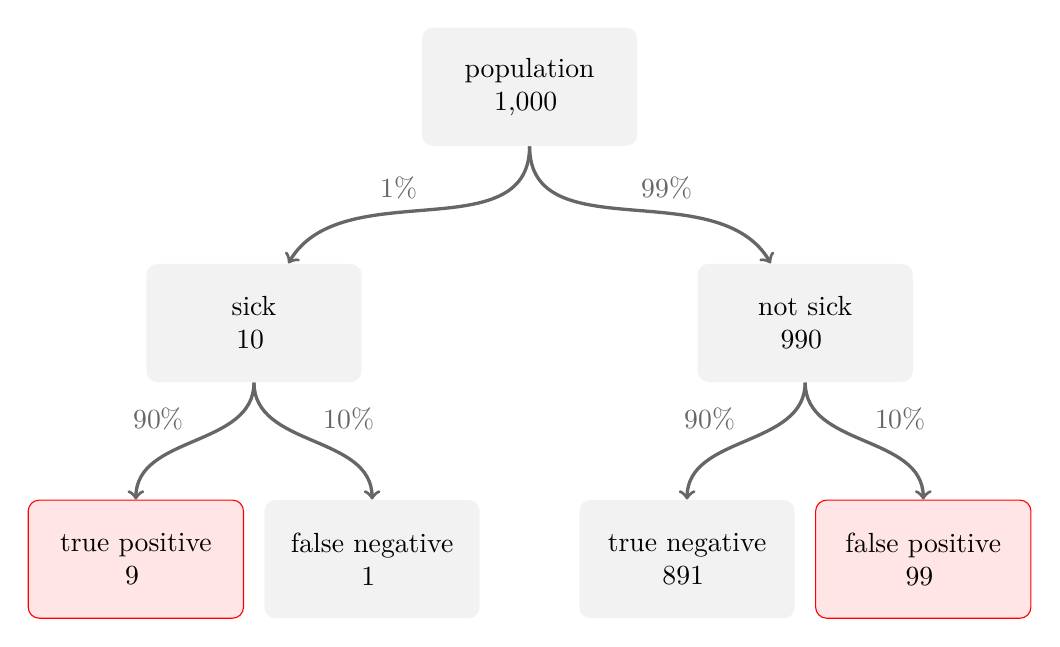
\begin{tikzpicture}
 \tikzset{block/.style={rectangle, text width=25mm, text centered, rounded corners, minimum height=1.5cm}};
%\draw [help lines] (-6,0) grid (6,6);%(0,0)から(10,4)までの"細線の方眼"
\node[block,fill=gray!10] (population) at (0,7) {population\\1,000人};
\pause
\node[block,fill=gray!10] (sick) at (-3.5,4) {sick\\10人};
\draw [->, very thick,color=black!60] (population) to[out=-90, in=60] node[auto=right] {有病率$1\%$} (sick); 
\pause
\node[block,fill=gray!10] (not_sick) at (3.5,4) {not sick\\990人};
\draw [->,very thick,color=black!60] (population) to[out=-90, in=120]  node[auto=left] {$99\%$} (not_sick); 
\pause
\node[block,fill=red!10,draw=red] (true_positive) at (-5,) {true positive\\9人};
\draw [->,very thick,,color=black!60] (sick) to[out=-90, in=90]  node[auto=right] {感度$90\%$} (true_positive); 
\pause
\node[block,fill=gray!10] (false_negative) at (-2,1) {false negative\\1人};
\draw [->,very thick,,color=black!60] (sick) to[out=-90, in=90]  node[auto=left] {$10\%$} (false_negative); 
\pause
\node[block,fill=gray!10] (true_negative) at (2,1) {true negative\\891人};
\draw [->,very thick,,color=black!60] (not_sick) to[out=-90, in=90]  node[auto=right] {特異度$90\%$} (true_negative); 
\pause
\node[block,fill=red!10,draw=red] (false_positive) at (5,1) {false positive\\99人};
\draw [->,very thick,,color=black!60] (not_sick) to[out=-90, in=90]  node[auto=left] {$10\%$} (false_positive); 
 \end{tikzpicture}%
}
\end{frame}

\begin{frame}{case study 1}
\protect\hypertarget{case-study-1-5}{}
\begin{center}\Huge               
\[
 \scalebox{1.4}{$\frac{9}{\;9 + 99\;}=0.08333$}
\]
\end{center}
\end{frame}

\begin{frame}{}
\protect\hypertarget{section-2}{}
\Huge

\scalebox{1.4}{\textcolor{softblue}{事例2}}
\end{frame}

\begin{frame}{case study 2 --- world war II}
\protect\hypertarget{case-study-2-world-war-ii}{}
\raggedleft

\IfFileExists{survivorship_bias.png}{\scalebox{.9}{\includegraphics{survivorship_bias.png}}}{\relax}

\tiny

\raggedleft

Martin Grandjean(vector), McGeddon(picture), Cameron Moll(concept)

\vspace{-5pt}

This work is licensed under the Creative Commons Attribution-Share Alike
4.0 International license.

\pause

\Huge
\vspace{-120pt}
\raisebox{120pt}{\rotatebox{10}{\textcolor{softblue}{\scalebox{1.2}{どこを}}}}

\vspace{-130pt}
\raisebox{130pt}{\rotatebox{10}{\textcolor{softblue}{\scalebox{1.2}{補強?}}}}
\end{frame}

\begin{frame}{case study 2 生存者のバイアス}
\protect\hypertarget{case-study-2-ux751fux5b58ux8005ux306eux30d0ux30a4ux30a2ux30b9}{}
\LARGE

データの偏り・欠落したデータ
\end{frame}

\begin{frame}{}
\protect\hypertarget{section-3}{}
\Huge

\scalebox{1.4}{\textcolor{softblue}{事例3}}
\end{frame}

\begin{frame}{case study 3}
\protect\hypertarget{case-study-3}{}
\Huge

\begin{itemize}
\item[\textbullet] ある自治体
\item[\textbullet] 複数の学校
\item[\textbullet] 共通学力テスト
\end{itemize}
\end{frame}

\begin{frame}{case study 3}
\protect\hypertarget{case-study-3-1}{}
\Huge

\begin{itemize}
\item[\textbullet] 試験勉強の時間
\item[\textbullet] 正答率
\end{itemize}
\pause
\vspace*{-55pt}
\rotatebox{20}{\scalebox{2}{\textcolor{softblue}{どんな関係?}}}
\end{frame}

\begin{frame}{plot}
\protect\hypertarget{plot}{}
\includegraphics{slide_files/figure-beamer/unnamed-chunk-4-1.pdf}
\end{frame}

\begin{frame}{case study 3}
\protect\hypertarget{case-study-3-2}{}
\includegraphics{slide_files/figure-beamer/unnamed-chunk-5-1.pdf}
\end{frame}

\begin{frame}{case study 3}
\protect\hypertarget{case-study-3-3}{}
\IfFileExists{./letsnotsee.jpg}{\centering\includegraphics[width=\textwidth]{./letsnotsee.jpg}}{\relax}
\end{frame}

\begin{frame}{case study 3}
\protect\hypertarget{case-study-3-4}{}
\includegraphics{slide_files/figure-beamer/unnamed-chunk-6-1.pdf}
\end{frame}

\begin{frame}{case study 3}
\protect\hypertarget{case-study-3-5}{}
\includegraphics{slide_files/figure-beamer/unnamed-chunk-7-1.pdf}
\end{frame}

\begin{frame}{case study 3}
\protect\hypertarget{case-study-3-6}{}
\includegraphics{slide_files/figure-beamer/unnamed-chunk-8-1.pdf}
\end{frame}

\begin{frame}{case study 3}
\protect\hypertarget{case-study-3-7}{}
\includegraphics{slide_files/figure-beamer/unnamed-chunk-9-1.pdf}
\end{frame}

\begin{frame}{case study 3}
\protect\hypertarget{case-study-3-8}{}
\includegraphics{slide_files/figure-beamer/unnamed-chunk-10-1.pdf}
\end{frame}

\begin{frame}{case study 3}
\protect\hypertarget{case-study-3-9}{}
\LARGE

\begin{itemize}
\item[\textbullet] 全体では\par
「勉強するほど成績がさがる」
\bigskip\pause
\item[\textbullet] 学校ごとでは\par
「勉強するほど成績があがる」
\end{itemize}
\end{frame}

\begin{frame}{case study 3 --- Simpson's Paradox}
\protect\hypertarget{case-study-3-simpsons-paradox}{}
\LARGE

全体と個々のグループでの傾向が異なる

\normalsize
\end{frame}

\begin{frame}{evidence-based policy-making}
\protect\hypertarget{evidence-based-policy-making-2}{}
\Huge

\raggedleft
\scalebox{2}{\textcolor{softblue}{データ}}\scalebox{1.2}{に基づき}

\scalebox{2}{\textcolor{lightpurple}{根拠}}\scalebox{1.2}{を持って}

\scalebox{1.2}{仕事を前に進めよう!}
\end{frame}

\begin{frame}{Part 2}
\protect\hypertarget{part-2}{}
\Huge

\scalebox{2}{\textcolor{lightpurple}{文書}}
\end{frame}

\begin{frame}{Sir Winston Spencer Churchill}
\protect\hypertarget{sir-winston-spencer-churchill}{}
\raggedleft\Huge

\raisebox{100pt}{\rotatebox{30}{\textcolor{white}{\scalebox{1.2}{Brevity}}}}  
\IfFileExists{Sir_Winston_Churchil.jpg}{\scalebox{.75}{\includegraphics{Sir_Winston_Churchil.jpg}}}{\relax}

\tiny

\raggedleft

The Roaring Lion(Yousuf Karsh) \vspace{-5pt}

This work is licensed under the Creative Commons Attribution 2.0 Generic
License.
\end{frame}

\begin{frame}{Sir Winston Spencer Churchill}
\protect\hypertarget{sir-winston-spencer-churchill-1}{}
\raggedleft\Huge

\raisebox{100pt}{\rotatebox{30}{\textcolor{black}{\scalebox{1.2}{Brevity}}}}  
\IfFileExists{Sir_Winston_Churchil.jpg}{\scalebox{.75}{\includegraphics{Sir_Winston_Churchil.jpg}}}{\relax}

\tiny

\raggedleft

The Roaring Lion(Yousuf Karsh) \vspace{-5pt}

This work is licensed under the Creative Commons Attribution 2.0 Generic
License.
\end{frame}

\begin{frame}{Brevity}
\protect\hypertarget{brevity}{}
\centering
\vspace*{-21.5pt}
\IfFileExists{churchill_memo.jpg}{\scalebox{1.025}{\includegraphics{churchill_memo.jpg}}}{\relax}
\end{frame}

\begin{frame}{Brevity}
\protect\hypertarget{brevity-1}{}
\Large

To do our work, we all have to read a mass of papers. Nearly all of them
are far too long.

\par

\vfill
\Huge

\rotatebox{15}{\scalebox{1.6}{\textcolor{white}{\begin{tabular}{l}大量の書類\\長すぎる\end{tabular}}}}

\vfill
\end{frame}

\begin{frame}{Brevity}
\protect\hypertarget{brevity-2}{}
\Large

To do our work, we all have to read
\textcolor{softblue}{a mass of papers}. Nearly all of them are
\textcolor{softblue}{far too long}.

\par

\vfill
\Huge

\rotatebox{15}{\scalebox{1.6}{\textcolor{softblue}{\begin{tabular}{l}大量の書類\\長すぎる\end{tabular}}}}

\vfill
\end{frame}

\begin{frame}{Brevity}
\protect\hypertarget{brevity-3}{}
\Large

This wastes time, while energy has to be spent in looking for the
essential points.

\par

\vfill\Huge

\rotatebox{15}{\scalebox{1.6}{\textcolor{white}{\begin{tabular}{l}時間のむだ\\要点がわからない\end{tabular}}}}

\vfill

\mbox{}
\end{frame}

\begin{frame}{Brevity}
\protect\hypertarget{brevity-4}{}
\Large

This \textcolor{softblue}{wastes time}, while energy has to be spent in
looking for \textcolor{softblue}{the essential points}.

\par

\vfill\Huge

\rotatebox{15}{\scalebox{1.6}{\textcolor{softblue}{\begin{tabular}{l}時間のむだ\\要点がわからない\end{tabular}}}}

\vfill
\end{frame}

\begin{frame}{Brevity}
\protect\hypertarget{brevity-5}{}
\Large

I ask my colleagues and their staffs to see to it that their Reports are
shorter.

\vfill\Huge

\rotatebox{15}{\scalebox{1.6}{\textcolor{white}{\begin{tabular}{l}報告書を短く\end{tabular}}}}

\vfill
\end{frame}

\begin{frame}{Brevity}
\protect\hypertarget{brevity-6}{}
\Large

I ask my colleagues and their staffs to see to it that
\textcolor{softblue}{their Reports are shorter}.

\vfill\Huge

\rotatebox{15}{\scalebox{1.6}{\textcolor{softblue}{\begin{tabular}{l}報告書を短く\end{tabular}}}}

\vfill
\end{frame}

\begin{frame}{Brevity}
\protect\hypertarget{brevity-7}{}
\Huge

\raggedleft
\scalebox{1.6}{文書は\scalebox{1.4}{\textcolor{softblue}{簡潔}}に!}
\end{frame}

\begin{frame}{Brevity}
\protect\hypertarget{brevity-8}{}
\Huge

\begin{itemize}
\item \scalebox{1.3}{歯切れよくいいきれ}
  \begin{itemize}
  \item \pause
  \item \scalebox{2}{\textbullet{}\myCrossedOut{softblue}{冗長ないいまわし}}
%  \item \scalebox{2}{\textbullet{}\myCrossedOut{softblue}{ぼかしことば}}
\end{itemize}
\end{itemize}
\end{frame}

\begin{frame}{Brevity}
\protect\hypertarget{brevity-9}{}
\LARGE
\scalebox{1.1}{AはBだと言ってよいのではないか}\par
\scalebox{1.1}{と思われる}
\end{frame}

\begin{frame}{Brevity}
\protect\hypertarget{brevity-10}{}
\LARGE

\scalebox{1.1}{AはBだと言ってよいのではないか}\par
\myCrossedOut{softred}{\scalebox{1.1}{と思われる}}
\end{frame}

\begin{frame}{Brevity}
\protect\hypertarget{brevity-11}{}
\LARGE

\scalebox{1.1}{AはBだと言ってよい\myCrossedOut{softblue}{のではないか}}\par
\myCrossedOut{softred}{\scalebox{1.1}{と思われる}}
\end{frame}

\begin{frame}{Brevity}
\protect\hypertarget{brevity-12}{}
\LARGE

\scalebox{1.1}{AはBだ\myCrossedOut{mintgreen}{と言ってよい}\myCrossedOut{softblue}{のではないか}}\par
\myCrossedOut{softred}{\scalebox{1.1}{と思われる}}
\end{frame}

\begin{frame}{Brevity}
\protect\hypertarget{brevity-13}{}
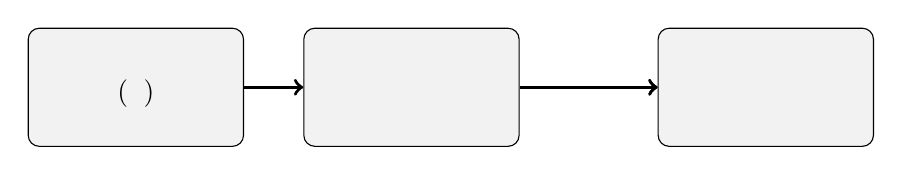
\begin{tikzpicture}
 \tikzset{block/.style={rectangle, text width=25mm, text centered, rounded corners, minimum height=1.5cm, fill=gray!10}};
  \node[draw, block] (factor1) at (0,0) {簡潔な文書\\(本質)};
  \pause
  \node[draw, block] (factor2) at (3.5,0) {明確な要点};
  \draw[->, very thick] (factor1) -- (factor2) node[midway, above] {};\pause
  \node[draw, block] (factor3) at (8,0) {迅速な \\意思決定};
 \draw[->, very thick] (factor2) -- (factor3) node[midway, above] {レク};
  \draw[->, very thick] (factor2) -- (factor3) node[midway, below] {決裁};
\end{tikzpicture}
\end{frame}

\begin{frame}{another important issue}
\protect\hypertarget{another-important-issue}{}
\LARGE
\raggedleft

\scalebox{1.4}{完成度の追求}\hspace{3.93pt}\mbox{}\pause

\vspace*{-35pt}

\scalebox{1.4}{\myCrossedOut{brightorange}{\textcolor{black}{完成度の追求}}}\pause

\scalebox{1.4}{8割でよし}\pause

\vfill

\scalebox{1}{でも数字や固有名詞}

\scalebox{1}{これだけはまちがえないぞ}
\end{frame}

\begin{frame}{}
\protect\hypertarget{section-4}{}
\Huge

\scalebox{1.2}{体裁}
\end{frame}

\begin{frame}{manual}
\protect\hypertarget{manual}{}
\vspace*{-20pt}
\IfFileExists{./tebiki.jpg}{\centering\scalebox{.9}{\rotatebox{-90}{\includegraphics[width=\textheight]{tebiki.jpg}}}}{\relax}
\end{frame}

\begin{frame}{quiz 1}
\protect\hypertarget{quiz-1}{}
\Huge

又は or または

\bigskip

\large

\raggedleft
\textcolor{white}{\begin{tabular}{@{}lll@{}}\toprule
教育振興基本計画&子供&手引のとおり\\
総合計画&子ども&手引から逸脱\\\bottomrule
\end{tabular}}

\vfill

\textcolor{white}{「子供と親のサポートセンター」とはいえない}
\end{frame}

\begin{frame}{quiz 2}
\protect\hypertarget{quiz-2}{}
\Huge

子供 or 子ども \pause

\bigskip

\large

\raggedleft
\begin{tabular}{@{}lll@{}}\toprule
教育振興基本計画&子供&手引のとおり\\\pause
総合計画&子ども&手引から逸脱\\\bottomrule
\end{tabular}
\pause

\vfill

「子供と親のサポートセンター」とはいえない
\end{frame}

\begin{frame}{quiz 3 ーter}
\protect\hypertarget{quiz-3-ux30fcter}{}
\Huge

\begin{tabular}{@{}ll@{}}
&コンピューター\\
or&コンピュータ
\end{tabular}

\pause

\vfill

\large
\raggedleft
\begin{tabular}{@{}ll@{}}\toprule
手引&原則「コンピューター」だが\\
&「コンピュータ」でもOK\\\pause
学習指導要領&「コンピュータ」\\\bottomrule
\end{tabular}
\pause

\vfill

「総合教育センタ」とはいえない
\end{frame}

\begin{frame}{手引 or 手引き}
\protect\hypertarget{ux624bux5f15-or-ux624bux5f15ux304d}{}
\IfFileExists{./seisaku_homu01.png}{\scalebox{1.05}{\includegraphics{seisaku_homu01.png}}}{\relax}
\end{frame}

\begin{frame}{manual}
\protect\hypertarget{manual-1}{}
\IfFileExists{./seisaku_homu03.png}{\scalebox{1.4018}{\includegraphics{seisaku_homu03.png}}}{\relax}
\end{frame}

\begin{frame}{tebiki}
\protect\hypertarget{tebiki}{}
\vspace*{-20pt}
\IfFileExists{./tebiki.jpg}{\centering\scalebox{.9}{\rotatebox{-90}{\includegraphics[width=\textheight]{tebiki.jpg}}}}{\relax}
\end{frame}

\begin{frame}{summing up}
\protect\hypertarget{summing-up}{}
\LARGE

\raggedleft
 \scalebox{1.4}{手引に従って}

\pause
\vfill

\scalebox{1.1}{でもほどほどに}
\end{frame}

\begin{frame}{I have a dream}
\protect\hypertarget{i-have-a-dream}{}
\LARGE

\scalebox{1.4}{\textcolor{black}{\begin{tabular}{l}私の夢は\\子供を笑顔にしたい\end{tabular}}}
\end{frame}

\begin{frame}{May this sign be displayed forever!}
\protect\hypertarget{may-this-sign-be-displayed-forever}{}
\vspace*{-4pt}
\IfFileExists{./bento.jpg}{\centering\scalebox{.85}{\includegraphics[width=\textheight]{bento.jpg}}}{\relax}
\end{frame}

\begin{frame}{}
\protect\hypertarget{section-5}{}
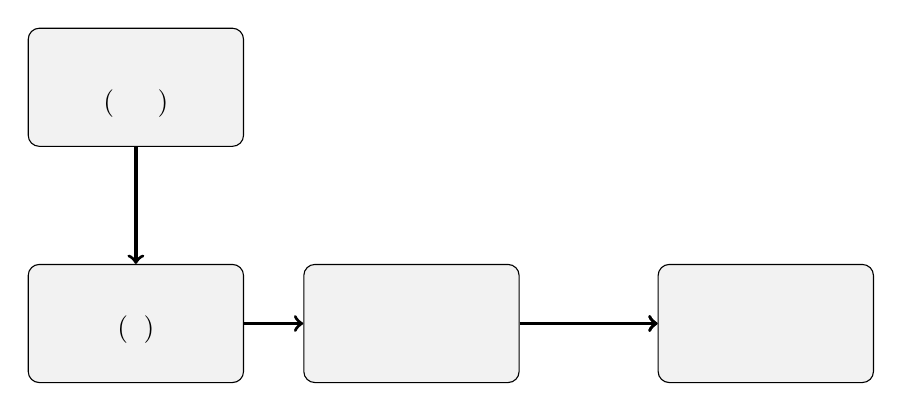
\begin{tikzpicture}
 \tikzset{block/.style={rectangle, text width=25mm, text centered, rounded corners, minimum height=1.5cm, fill=gray!10}};
  \node[draw, block] (factor0) at (0, 3) {\begin{tabular}{@{}l@{}}根拠\\{(\footnotesize 法令・データ等})\end{tabular}};
  \node[draw, block] (factor1) at (0,0) {簡潔な文書\\(本質)};
  \draw[->, very thick] (factor0) -- (factor1) node[midway, right] {整理}; 
  \node[draw, block] (factor2) at (3.5,0) {明確な要点};
  \draw[->, very thick] (factor1) -- (factor2) node[midway, above] {};
  \node[draw, block] (factor3) at (8,0) {迅速な \\意思決定};
   \draw[->, very thick] (factor2) -- (factor3) node[midway, above] {レク};
  \draw[->, very thick] (factor2) -- (factor3) node[midway, below] {決裁};
\end{tikzpicture}

\vfill

\raggedleft

文書のできは8割でよし

体裁は手引どおりに。でも、ほどほどに
\end{frame}

\begin{frame}[fragile]{}
\protect\hypertarget{section-6}{}
\begin{Shaded}
\begin{Highlighting}[]
\FunctionTok{piyopiyo}\NormalTok{()}
\end{Highlighting}
\end{Shaded}

\includegraphics{slide_files/figure-beamer/cars-1.pdf}
\end{frame}

\end{document}
